\section{FS Transfer Protocol}

    Depois do \textit{tracker} fornecer todas as informações necessárias à aquisição dos ficheiros pretendidos, o cliente pode iniciar de imediato o processo de transferência com os restantes nós.

    Tal como para o protocolo anterior, também neste caso definimos um segmento capaz de suportar todas as informações necessárias à transferência de ficheiros, o que por sua vez facilita bastante o desenvolvimento de código, no sentido em que apenas uma estrutura de dados é serializada/deserializada.

    Fora isso, e tendo em consideração que os segmentos são enviados a partir de um \textit{datagram socket}, torna-se evidente a necessidade de existirem campos que permitam o controlo de fluxo e erros.

    \newpage
    \begin{figure}[hb!]
        \centering
        \includegraphics[width=0.45\textwidth]{Imagens/Headers/node.png}
        \caption{Cabeçalho de um \textit{UDPPacket}}
    \end{figure}

    O cabeçalho apresentado é bastante semelhante ao de um \textit{TCPPacket}, excetuando os campos \textit{Número de Sequência} (possibilita a ordenação dos blocos) e \textit{Checksum} (permite a identificação de erros).

    A presença dos campos \textit{IP} e \textit{Porta Origem} pode levantar algumas questões, visto que por norma estes seriam facilmente obtidos através de métodos que a própria linguagem de programação disponibiliza, todavia acreditamos que desta forma obtemos uma implementação mais robusta e independente.

    \subsection{Threads}

        Um cliente pode ser contactado a qualquer momento pelos restantes, como tal é necessário atender os pedidos e fornecer as respetivas respostas. Tendo isto em mente, cada cliente possui uma \textit{thread} à escuta numa determinada porta que é conhecida \textit{a priori} por todos os nós da rede.

        Depois de receber e analisar um determinado segmento, o cliente em questão deve assegurar uma resposta, contudo não pode permitir que outros pedidos fiquem por atender, como tal é necessário criar uma nova \textit{thread} cuja função será única e exclusivamente retorquir o pedido em causa.

        A princípio pensámos que seria uma mais-valia criar uma \textit{thread pool}, visto que isso permite a reutilização de \textit{threads}, contudo reparámos que a \textit{thread} principal poderia bloquear caso o tamanho do \textit{buffer} fosse relativamente pequeno quando comparado com a quantidade de nós na rede.

        Ao definirmos que um pedido dá origem a uma \textit{thread}, obtemos um programa significativamente menos eficiente, contudo garantimos que ninguém irá bloquear, seja em que situação for.

        \newpage
        \begin{figure}[hb!]
            \centering
            \includegraphics[width=0.75\textwidth]{Imagens/Estruturas/threads.png}
            \caption{Arquitetura do atendimento de pedidos}
        \end{figure}    

    \subsection{Funcionamento}

        Tendo a noção de como os pedidos são atendidos, e conhecendo perfeitamente a estrutura de um \textit{UDPPacket}, podemos especificar o comportamento normal da comunicação entre dois clientes, a fim de um deles obter um determinado conjunto de blocos.

        \begin{enumerate}
            
            \item O cliente \textit{A} envia um \textit{UDPPacket} cujo protocolo corresponde a \textit{HELLO}.

            \item O cliente \textit{B} recebe o segmento e percebe que o \textit{A} quer contactar consigo.

            \item O cliente \textit{B} cria uma \textit{thread} que irá responder ao \textit{A}.

            \item O cliente \textit{B} envia um \textit{UDPPacket} com protocolo \textit{HELLO}, indicando a porta que deverá ser utilizada.

            \item O cliente \textit{A} envia vários \textit{GET's} que contêm os identificadores dos blocos que pretende obter.

            \item O cliente \textit{B} recebe os segmentos e recolhe os blocos pretendidos pelo cliente \textit{A}.

            \item O cliente \textit{B} envia diversos \textit{DATA's} com as informações dos blocos.

            \item O cliente \textit{A} percebe que possui todos os blocos requisitados e escreve-os em disco.

            \item O cliente \textit{A} anuncia ao \textit{tracker} que possui um ficheiro novo.

        \end{enumerate}
        
        \newpage
        \begin{figure}[hb!]
            \centering
            \includegraphics[width=0.75\textwidth]{Imagens/Diagramas Temporais/node.png}
            \caption{Diagrama temporal da comunicação entre clientes}
        \end{figure}

    \subsection{Sliding Window}

        A utilização de \textit{datagram sockets} não assegura que os segmentos enviados cheguem de facto ao seu destino, como tal é necessário estabelecer um pequeno algoritmo que permita isso mesmo, algoritmo esse que se baseia fundamentalmente nos seguintes pontos.

        \begin{itemize}
            
            \item A receção de um segmento é confirmada com o envio de um \textit{acknowledgement}.

            \item A não receção de um \textit{acknowledgement} implica necessariamente que o segmento não chegou corretamente.

            \item Depois de receber todos os \textit{acknowledgements} expectáveis, o emissor aborta o envio de segmentos.

            \item Ao não receber nenhum segmento, o recetor conclui que o emissor já enviou tudo.

            \item O \textit{timeout} do recetor é bastante superior ao do emissor, não permitindo que este seja induzido em erro.
            
        \end{itemize}

        Com estes pontos bem assentes, podemos definir uma versão do algoritmo de \textit{sliding window} utilizado pelo TCP. Ao analisarmos esta estratégia, verificámos que à partida era enviada uma determinada quantidade de segmentos \textit{(window size)}, contudo, a partir daí, havia uma certa tendência para bloqueios, visto ser necessário receber o \textit{acknowledgement} do elemento que estava na primeira posição da janela.

        Esta situação parece-nos um pouco estranha e desnecessária, portanto a nossa versão do \textit{sliding window} procura corrigir essa tendência para bloqueios.

        \begin{wrapfigure}{r}{0.4\textwidth}
            \begin{center}
            \vspace{-25pt}
            \includegraphics[width=0.4\textwidth]{Imagens/Estruturas/node blocos.png}
            \caption{\textit{Buffer} de blocos}
            \vspace{-50pt}
            \end{center}
        \end{wrapfigure}

        \hspace{4.5pt}1.~ O emissor define um \textit{timeout} bastante inferior ao do recetor.

        \hspace{4.5pt}2.~ O emissor criar um \textit{buffer} onde constam os segmentos.
            
        \hspace{4.5pt}3.~ O emissor envia uma determinada quantidade de segmentos.
        
        \hspace{4.5pt}4.~ O emissor aguarda a chegada de um \textit{acknowledgement}.

        \hspace{4.5pt}5.~ A receção de uma confirmação apaga um segmento do \textit{buffer.}

        \hspace{4.5pt}6.~ O emissor envia outro segmento e repete os passos 4 e 5.

        \hspace{4.5pt}7.~ Depois de enviar o último segmento, volta ao início.

        \hspace{4.5pt}8.~ O processo termina quando todas as confirmações chegarem.

        \begin{wrapfigure}{r}{0.4\textwidth}
            \begin{center}
                \vspace{-25pt}
                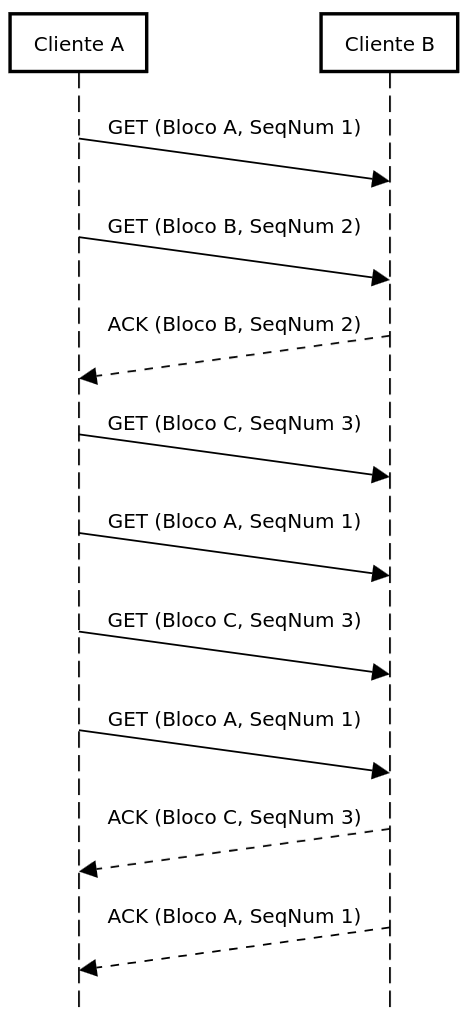
\includegraphics[width=0.35\textwidth]{Imagens/Diagramas Temporais/udp.png}
                \caption{Diagrama temporal}
                \vspace{-50pt}
            \end{center}
        \end{wrapfigure}

        Ao analisarmos o diagrama temporal correspondente ao envio de segmentos, percebemos claramente a vantagem desta reformulação do algoritmo de \textit{sliding window}.

        Supondo uma janela de tamanho dois, originalmente o algoritmo começa por enviar dois segmentos \textit{(A e B)}, todavia, para poder prosseguir, é necessário que chegue o \textit{acknowledgement} do segmento \textit{A}, algo que não acontece.

        Posto isto, a janela iria ficar bloqueada até que o \textit{acknowledgement} desejado chegasse, o que não é minimamente aconselhável se queremos tirar o máximo partido da rede.

        Assim sendo, na nossa implementação, a janela continua a deslizar sem se preocupar que os segmentos tenham sido corretamente enviados, visto que após chegar ao fim do \textit{buffer}, o processo irá repetir-se de modo a que os segmentos não confirmados sejam retransmitidos.

        Apesar de promissora, esta solução acaba por criar um novo problema capaz de saturar qualquer rede num instante. Embora um segmento tenha chegado corretamente ao seu destino, o mesmo será retransmitido várias vezes, pois o \textit{timeout} do emissor é demasiado curto, o que origina imensas replicações de dados.

    \subsection{Controlo de Erros}

        A utilização de \textit{datagram sockets} não garante vários aspetos, entre eles a integridade dos segmentos, como tal é necessário definir uma estratégia que permita ao recetor perceber se uma dada mensagem foi corrompida.

        A princípio pensámos em utilizar \textit{SHA-1}, todavia percebemos que essa função de \textit{hash} não era apropriada para efetuar controlo de erros, sendo um dos motivos apontados a complexidade que o algoritmo exige.

        Desta forma, é fundamental procurar um balanço entre a eficácia na detenção de erros, e a complexidade na criação do \textit{hash}, assim sendo, chegámos a um algoritmo designado de \textit{CRC32C}, que pelos vistos é o sucessor do \textit{CRC32} utilizado pelo \textit{layer 2}.

        Após efetuarmos a transferência de milhões de segmentos entre nós do \textit{CORE}, verificámos que o nosso algoritmo de deteção de erros não foi ativado uma única vez, o que nos levou a formular algumas hipóteses.

        \begin{itemize}
            
            \item Será que o controlo de erros efetuado pelas camadas inferiores foi tão eficaz ao ponto de não detetarmos qualquer erro no nível aplicacional?

            \item Será que a linguagem de programação utilizada garante a integridade dos dados caso eles cheguem ao seu destino?

        \end{itemize}

        A primeira hipótese não tem grande credibilidade, portanto fomos ler de imediato a documentação do \textit{Java}, e tendo em conta que este tema não estava mencionada nos avisos sobre a utilização de \textit{datagram sockets}, a segunda hipótese é afinal verdadeira, pelo que o controlo de erros é realizado implicitamente.